\documentclass[
 reprint,
 amsmath,amssymb,
 aps,
 prb,
]{revtex4-2}

\usepackage{graphicx}
\usepackage{bm}

\usepackage{physics}

\usepackage[colorlinks=true,
            linkcolor=blue,
            filecolor=blue,
            urlcolor=blue,
            citecolor=blue]{hyperref}

\usepackage{caption}
\captionsetup[figure]{
    justification=raggedright,
    labelfont={bf},
    name={Fig.},
    labelsep=period
}
\captionsetup[table]{
    labelfont={bf},
    name={Table},
    labelsep=period
}

\numberwithin{equation}{section}

\tolerance=1000
\emergencystretch=1em
\hyphenpenalty=3000
\exhyphenpenalty=3000
\flushbottom

\usepackage[final]{microtype}

\usepackage{ragged2e}  

\usepackage{booktabs}

\usepackage{amsthm}
\newtheorem{theorem}{Theorem}[section]

\usepackage{listings}
\usepackage{xcolor}

\definecolor{backcolour}{rgb}{0.96,0.97,0.98}
\definecolor{deepblue}{rgb}{0,0,0.5}
\definecolor{deepgreen}{rgb}{0,0.5,0.3}
\definecolor{deepgray}{rgb}{0.4,0.4,0.4}
\definecolor{stringcolor}{rgb}{0.2,0.4,0.6}

\lstdefinestyle{pythonstyle}{
    backgroundcolor=\color{backcolour},
    commentstyle=\color{deepgreen}\itshape,
    keywordstyle=\color{deepblue}\bfseries,
    numberstyle=\tiny\color{deepgray},
    stringstyle=\color{stringcolor},
    basicstyle=\ttfamily\footnotesize,
    breakatwhitespace=false,
    breaklines=true,
    captionpos=b,
    keepspaces=true,
    numbers=left,
    numbersep=5pt,
    showspaces=false,
    showstringspaces=false,
    showtabs=false,
    tabsize=2,
    language=Python,
    frame=single,
    rulecolor=\color{deepgray}
}
\lstset{style=pythonstyle}

\newcommand{\iphase}{\theta}  

\usepackage{tikz}
\usetikzlibrary{arrows.meta, calc, 3d, shadings, positioning, decorations.pathmorphing}

\begin{document}

\title{Geometrical Confinement of Energy in the 0-Sphere Model:\\
A Topological Mechanism Underlying Rest Mass,\\
Zitterbewegung, and Gravitational-Like Phenomena\\[0.5ex]
\normalsize --- Emergent Gravitational Dynamics Without Additional Mediators}

\author{Satoshi Hanamura}
\email{hana.tensor@gmail.com}
\date{January 31, 2026}

\begin{abstract}
We present a fully self-contained extension of the 0-Sphere model that provides the first explicit derivation of gravitational-like phenomena from topological and thermodynamic principles. Unlike conventional field theories, interactions emerge from line integrals of phase histories, eliminating the need for continuous spacetime fields or unobserved gravitons. Internal oscillations within atoms or molecules, represented as effective 0-Sphere subsystems, undergo entropic synchronization mediated by photon exchange. This process results in emergent drift motion and effective free-fall acceleration, without introducing any mediator beyond the photon. Quantitative predictions for microscopic realizations using trapped quantum oscillators are provided, establishing a framework for experimental verification and potential unification of inertia, gravitation, and quantum phase dynamics. Idealized estimates indicate that the cumulative photon-mediated phase synchronization can produce accelerations comparable to Earth's gravity, establishing a quantitative link between microscopic oscillatory dynamics and macroscopic gravitational-like behavior. This yields quantitative agreement with gravitational-scale accelerations and establishes a numerical bridge between quantum phase dynamics at the Compton wavelength scale and macroscopic gravity. This work is intended not only as a physical proposal, but also as a structured reference point for evaluating emergent-force models based on phase, energy flow, and information transfer.
\end{abstract}

\maketitle

\section{Introduction}
\label{sec:introduction}

Traditional physical theories, such as general relativity (GR) \cite{Einstein1916} and quantum field theory (QFT), rely on continuous fields defined at every point in spacetime. In GR, gravitational interactions arise from spacetime curvature, while in QFT, forces emerge as gradients of local fields. Despite their success, these frameworks implicitly assume dense, unobservable coordinate markers and do not specify a microscopic mechanism for the emergence of inertia or gravitational acceleration.

The 0-Sphere model ~\cite{Hanamura2025Trilogy1,Hanamura2026Trilogy2,Hanamura2026Trilogy3} provides an alternative by replacing pointwise field values with topological entities that represent spinorial particles with intrinsic oscillatory degrees of freedom. In earlier work, the 0-Sphere formalism was primarily applied to internal degrees of freedom within a single electron, where each electron contains two discrete energy kernels undergoing rapid internal oscillations, or Zitterbewegung \cite{Schrodinger1930,Dirac1928,Barut1981}. In the present study, the framework is extended to encompass composite matter systems, such as atoms or molecules, whose internal phase dynamics can be effectively modeled within the same spinorial description. The electron-level realization remains as a special case within this extended framework. Each atom or molecule inherits the internal oscillatory structure from its constituent electrons and nucleons, collectively exhibiting phase dynamics represented by a variable $\theta(t)$. The history of these oscillations is encoded as a \textit{line integral} over trajectories in an abstract embedding space. Crucially, phase-mediated interactions between matter constituents are not mediated by classical fields, but through a \textit{phase network}—a spacetime mesh constructed from cumulative phase histories encoded in photon-mediated exchanges between neighboring atoms or molecules. Physical effects, including emergent acceleration, are therefore a consequence of the topology and thermodynamic evolution of these phase histories rather than local gradients \cite{Hanamura2026Trilogy3,AharonovBohm1959,Berry1984,WilsonLoop1974}.

This work extends the 0-Sphere framework to phenomena traditionally associated with gravity. We demonstrate that free-fall motion and apparent forces emerge from \textit{entropic entrainment}: a thermodynamically favorable synchronization of internal oscillations mediated by photon exchange between matter constituents \cite{Pikovsky2001,Strogatz2000,Bennett2002}. An effective 0-Sphere subsystem adjusts its internal frequency to match the ambient phase network constructed from neighboring subsystems, maximizing entropy and minimizing free energy. The energy released in this process, $\Delta E_\text{vib}$, is converted to translational kinetic energy $E_\text{kin}$, producing motion toward the phase ensemble. This entropic synchronization is mediated by photon exchange, which propagates at light speed, enforcing causality. Unlike prior models, no continuous gravitational field or hypothetical gravitons are required.

By explicitly stating all previously implicit assumptions—line-integral mediation, photon-based communication between matter constituents, entropic synchronization, and frictionless idealization—this model provides a quantitative bridge between microscopic Zitterbewegung and macroscopic free-fall motion. It offers a foundation for a unified perspective on inertia, gravitation, and quantum phase dynamics \cite{Jacobson1995,Verlinde2011,Padmanabhan2010}, and it allows experimentally testable predictions at microscopic scales.

In particular, if inertial mass is understood as arising from internal oscillatory energy flow, then phase synchronization between matter constituents requires no interaction channel beyond photon exchange, allowing gravitational-like behavior to be addressed within known physical degrees of freedom.

This perspective naturally raises the possibility that phenomena traditionally attributed to gravity may be accounted for without introducing an independent gravitational mediator, relying instead on phase synchronization mediated by photons within known physical frameworks.

\subsection*{Outline}

The remainder of this paper is organized as follows. In Sec.~\ref{sec:theory}, we introduce the extended 0-Sphere formalism and define the internal phase variables, line-integral histories, effective subsystem description, entropic entrainment mechanism, and photon-mediated phase communication used throughout the analysis. Sec.~\ref{sec:math} develops the mathematical framework of line-integral-based interactions and provides predictive formulas for energy conversion and effective acceleration. Sec.~\ref{sec:idealized_simulation} presents an idealized numerical simulation illustrating the emergence of free-fall–like motion under noise-free conditions. Finally, Sec.~\ref{sec:conclusion} summarizes the results and discusses their implications for inertia, gravitation, and emergent dynamics within known physical degrees of freedom.

\section{Theoretical Model}
\label{sec:theory}

\subsection{Scope and Theoretical Stance}

\subsubsection{Theoretical Stance and Nonlocality}

Before introducing the specific elements of the extended 0-Sphere formalism, it is important to clarify the theoretical stance adopted in this work. The 0-Sphere model is \emph{not} formulated as a local field theory. Physical effects are not derived from pointwise field values, spatially defined force gradients, or differential field equations imposed over spacetime. Instead, the primary physical objects are \emph{line integrals of phase histories}, or loci, accumulated along admissible trajectories that connect discrete energy-localized subsystems.

In this framework, interaction is intrinsically history-dependent. Observable effects arise from the cumulative phase acquired through photon-mediated emission and absorption processes, encoded as open-path line integrals. This standpoint builds directly on earlier work in which line integrals were identified as fundamental physical observables, unifying the Aharonov--Bohm effect, Berry phase, and Wilson-loop--type constructions within a single integral-based ontology~\cite{Hanamura2026Trilogy3}. The present paper does not revisit the foundational justification of this ontology, but adopts it as a working premise to investigate emergent gravitational-like behavior in composite systems. Accordingly, all subsequent notions of interaction, synchronization, force, and acceleration should be understood as emergent consequences of line-integral phase histories and their thermodynamic evolution, rather than as manifestations of underlying continuous fields defined on spacetime.

\subsubsection{Spatial Structure, Photon Sphere, and Thermal Geodesics}

At the same time, the rejection of local field descriptions does not imply the absence of spatial localization or finite geometric structure. In the 0-Sphere model, even a single electron is described by two discrete energy kernels, denoted kernel $A$ and kernel $B$, corresponding to the two points of the 0-sphere $S^{0}$. As established in earlier work, these kernels are localized in physical space and are separated by a characteristic distance of the order of the electron Compton wavelength~\cite{Hanamura2026Trilogy3}. At a fundamental level, this asymmetry does not correspond to a spatial gradient defined over physical space, nor does it introduce a local force field acting on the particle. The finite separation between kernel $A$ and kernel $B$ therefore does not define a local force or potential gradient acting between them.

An important distinction concerns the physical status of the photons involved. The photon-mediated phase communication in the 0-Sphere model is realized through \emph{real}, on-shell photons, not the virtual photons of perturbative quantum field theory. Virtual photons are off-shell mathematical constructs appearing in Feynman diagrams and serve as computational devices rather than observable physical entities. By contrast, the photons responsible for phase synchronization in the present framework are real quanta propagating at the speed of light, carrying energy--momentum together with geometric phase information along their worldlines. This distinction allows gravitational-like behavior to emerge from established physical degrees of freedom, without invoking additional unobserved mediators such as gravitons. Accordingly, the photon sphere should be understood as a geometrically structured collection of real photon trajectories encoding cumulative phase histories, rather than as a continuum of virtual particle exchanges.

A natural question arises: if real photons are emitted during phase communication between subsystems, does the photon sphere surrounding each kernel pair become depleted? The answer lies in the thermodynamic nature of the photon ensemble. Unlike matter particles, photons do not conserve chemical potential ($\mu = 0$ in thermal equilibrium), meaning the photon number is not a conserved quantity. As photons are emitted to mediate inter-subsystem phase synchronization, new photons are continually generated through internal oscillatory dynamics to maintain thermal equilibrium within each effective 0-Sphere subsystem. The photon sphere is therefore not a finite reservoir that becomes exhausted, but rather a dynamically sustained state characterized by continuous emission, absorption, and regeneration processes. This thermodynamic property ensures that phase-mediated interactions can persist indefinitely without depleting the internal structure of participating subsystems.

As an intuitive analogy, one may consider a water droplet in microgravity: when smaller droplets merge with a larger one, the combined system forms a single droplet held together by surface tension, capable of sustaining internal oscillatory modes characterized by spherical harmonics $Y_{\ell m}(\theta,\phi)$. Similarly, the photon sphere is a dynamically sustained geometric structure that absorbs and emits photons while maintaining its overall form through continuous regeneration, without requiring photon number conservation. This analogy illustrates how a stable structure can persist without an associated conserved particle number, though it does not imply material equivalence between water droplets and photon ensembles.

All admissible transport, phase accumulation, and radiative exchange occur exclusively through an embedding into an arcwise connected domain, interpreted physically as the photon sphere. The photon sphere is not a continuous field defined at every point, but rather a geometrically characterized collection of admissible radiative paths along which line integrals can be defined. This embedding provides the arcwise connectivity necessary for path-dependent phase accumulation, without requiring pointwise field assignments between the kernels. Within this embedding region, continuous radiative paths exist and support line-integral observables, while the kernels themselves remain fixed endpoints of the process. No continuous field is assigned to individual points of the photon sphere or to the region directly connecting the kernels. Instead, the photon sphere provides only the topological structure---specifically, arcwise connectivity---necessary to support one-dimensional line integrals along thermally realized trajectories.

These trajectories correspond to the thermal geodesics established in earlier work~\cite{Hanamura2025Trilogy1}, which provide the geometric framework for energy transport between kernels, parametrized by proper time $\tau$ to ensure observer independence. The fundamental observables---accumulated geometric phase along these thermal geodesics---are defined strictly along one-dimensional worldlines regardless of the dimension of the embedding manifold, consistent with the dimensional independence principle~\cite{Hanamura2025Trilogy1}. In the present extension to composite systems, such as atoms or molecules modeled as effective 0-Sphere subsystems, thermal geodesics are physically realized through photon emission and absorption processes that mediate both energy transfer and phase information exchange between neighboring subsystems. Photons thus encode the accumulated history of oscillatory dynamics along the thermal geodesic structure.

The finite spatial separation between kernel $A$ and kernel $B$ therefore enters the theory only through its role in setting the geometric scale of admissible radiative paths and the associated phase accumulation along those paths. All dynamical effects arise from the history of photon-mediated transport within the embedding domain and its synchronization with other effective subsystems, fully consistent with the line-integral--based ontology adopted throughout this work.

\begin{figure*}[t!]
\centering 
\resizebox{\textwidth}{!}{%
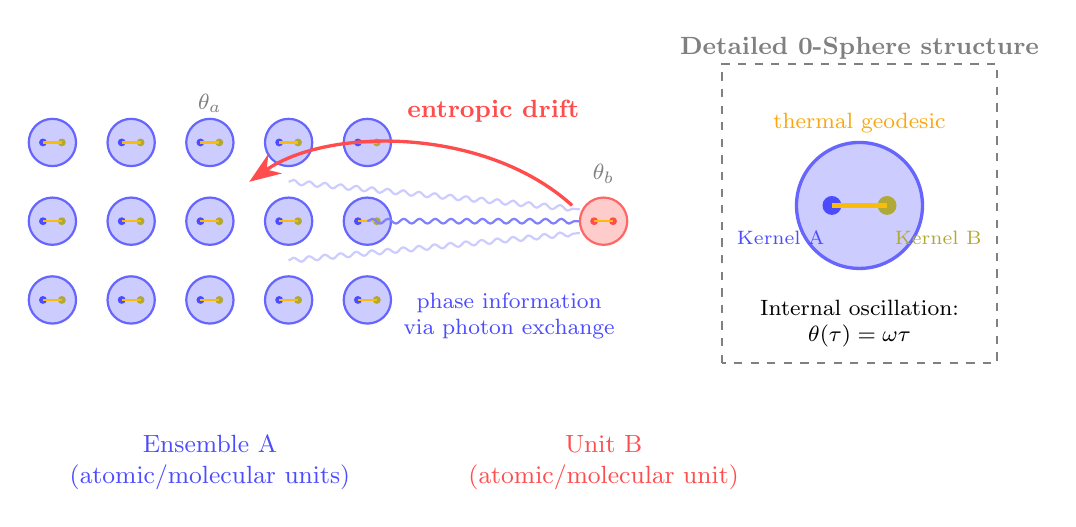
\begin{tikzpicture}
% Ensemble A - atoms/molecules with internal 0-Sphere structure
\foreach \x in {-2,-1,0,1,2} {
  \foreach \y in {-1,0,1} {
    % Outer circle
    \draw[fill=blue!20, draw=blue!60, thick] (\x,\y) circle (0.3);
    % Two discrete kernels
    \fill[blue!70] (\x-0.12,\y) circle (0.05);
    \fill[olive!70] (\x+0.12,\y) circle (0.05);
    % Thermal geodesic (yellow)
    \draw[yellow!50!orange, thick] (\x-0.12,\y) -- (\x+0.12,\y);
  }
}
% Single subsystem B
\draw[fill=red!20, draw=red!60, thick] (5,0) circle (0.3);
\fill[red!70] (5-0.12,0) circle (0.05);
\fill[red!70] (5+0.12,0) circle (0.05);
\draw[yellow!50!orange, thick] (5-0.12,0) -- (5+0.12,0);
% Internal phase labels
\node[font=\footnotesize, gray, fill=white, inner sep=1pt, opacity=0.8, text opacity=1] 
      at (0,1.5) {$\theta_a$};
\node[font=\footnotesize, gray, fill=white, inner sep=1pt, opacity=0.8, text opacity=1] 
      at (5,0.6) {$\theta_b$};
% Entropic drift arrow
\draw[-{Stealth[length=4mm]}, very thick, red!70] 
      (4.6,0.2) .. controls (3.5,1.2) and (1.5,1.2) .. (0.5,0.5);
\node[red!70, font=\small\bfseries] at (3.6,1.4) {entropic drift};
% Photon-mediated interactions
\draw[decorate, decoration={snake, amplitude=0.3mm, segment length=2mm}, 
      blue!50, thick] (2,0) -- (4.7,0);
\draw[decorate, decoration={snake, amplitude=0.3mm, segment length=2mm}, 
      blue!50, thick, opacity=0.4] (1,0.5) -- (4.7,0.15);
\draw[decorate, decoration={snake, amplitude=0.3mm, segment length=2mm}, 
      blue!50, thick, opacity=0.4] (1,-0.5) -- (4.7,-0.15);
\node[blue!70, font=\footnotesize, align=center, fill=white, inner sep=2pt] 
     at (3.8,-1.2) {phase information\\via photon exchange};
% Zoomed inset
\draw[gray, dashed, thick] (6.5,-1.8) rectangle (10.0,2.0);
\node[gray, font=\small\bfseries] at (8.25,2.2) {Detailed 0-Sphere structure};
% Zoomed 0-Sphere
\draw[fill=blue!20, draw=blue!60, very thick] (8.25,0.2) circle (0.8);
\fill[blue!70] (8.25-0.35,0.2) circle (0.12);
\fill[olive!70] (8.25+0.35,0.2) circle (0.12);
\draw[yellow!50!orange, ultra thick] (8.25-0.35,0.2) -- (8.25+0.35,0.2);
% Zoom labels
\node[blue!70, font=\scriptsize, below] at (8.25-1.0,0.0) {Kernel A};
\node[olive!70, font=\scriptsize, below] at (8.25+1.0,0.0) {Kernel B};
\node[font=\footnotesize, yellow!30!orange, above] 
     at (8.25,1.0) {thermal geodesic};
\node[font=\footnotesize, align=center] 
     at (8.25,-1.3) {Internal oscillation:\\$\theta(\tau) = \omega \tau$};
% Bottom labels
\node[blue!70, font=\small, below, align=center] 
     at (0,-2.6) {Ensemble A\\(atomic/molecular units)};
\node[red!70, font=\small, below, align=center] 
     at (5,-2.6) {Unit B\\(atomic/molecular unit)};
\end{tikzpicture}
}
\caption{\justifying
Schematic representation of effective 0-Sphere subsystems interpreted as atomic or molecular units with internal phase dynamics. Each unit (outer circle) contains two discrete energy kernels (dots) connected by a thermal geodesic (yellow line segment), representing the effective 0-Sphere structure in the sense of the present model. In this work, the 0-Sphere model is assumed to describe primarily \textit{electrons} within atoms and molecules, which are the dominant carriers of energy in photon-mediated interactions. Photon-mediated coupling to protons or neutrons is negligible at the energy scales relevant to atomic and molecular dynamics and is not included in this representation. Ensemble A is drawn with all kernels aligned for clarity; in reality, each kernel's orientation depends on its spin state and can point in arbitrary directions. Unit B (red, internal phase $\theta_b$) undergoes entropic drift toward the synchronized ensemble A (blue, internal phase $\theta_a$). Phase information is exchanged via emitted and absorbed photons (wavy lines), mediating synchronization without invoking continuous gravitational fields. The inset shows the detailed 0-Sphere structure: two discrete energy kernels connected by a thermal geodesic (yellow), along which the internal phase $\theta(\tau) = \omega \tau$ accumulates.
}
\label{fig:entrainment}
\end{figure*}

\subsection{0-Sphere Structure and Internal Oscillations}

In this work, a ``0-Sphere'' does not denote an elementary particle in the conventional sense, but rather an effective description of internal oscillatory degrees of freedom associated with matter constituents, such as atoms or molecules. Each effective 0-Sphere subsystem represents a localized spinorial entity that carries internal phase dynamics and can exchange phase information via photon-mediated interactions.

At the single-electron level, this structure consists of two discrete energy kernels separated by the Compton wavelength
\begin{equation}
\lambda_C = \frac{\hbar}{m_e c},
\label{eq:compton_wavelength}
\end{equation}
connected by radiative exchange through an internal photon sphere. Energy circulates between these kernels with characteristic frequency $\omega \sim m_e c^2/\hbar$, establishing an internal geometric phase $\theta(t) = \omega t/2$ and an associated SU(2) spinorial structure. The internal circulation gives rise to observable properties including spin, anomalous magnetic moment, and Zitterbewegung dynamics. The characteristic Zitterbewegung velocity $v_\text{zb} \simeq 0.04c$ has been derived from energy conservation and relativistic kinematics in earlier work~\cite{Hanamura2024Quantum}.

For composite systems such as atoms or molecules modeled as effective 0-Sphere subsystems, the oscillatory structure is inherited from constituent electrons and nucleons, collectively exhibiting phase dynamics that can be represented by an effective phase variable $\theta(t)$~\cite{Hanamura2026Trilogy3,Hanamura2025Trilogy1}. The oscillation frequency is denoted $\nu_k$, corresponding to internal vibrational energy $E_\text{vib} = \hbar \nu_k$. These oscillations are quasi-periodic and localized within each atom or molecule, yet capable of interacting with surrounding matter constituents through the phase network. Zitterbewegung~\cite{Schrodinger1930,Dirac1928,Barut1981} is interpreted here as a candidate microscopic carrier of internal energy at the atomic and molecular scale. Within the entropic framework adopted in this work, these internal oscillatory dynamics may contribute to emergent inertial behavior and phase-mediated interactions between matter constituents.

\subsection{Phase Network and Line-Integral Mediation}

The \textit{phase network} is a history-dependent structure constructed from cumulative oscillation histories of surrounding effective 0-Sphere subsystems \cite{Hanamura2026Trilogy3}. Let $\gamma$ denote the trajectory of an effective subsystem in the network. The effective interaction is determined by the line integral
\begin{equation}
\Delta \theta_\text{eff} = \int_\gamma d\theta,
\label{eq:line_integral}
\end{equation}
which encodes the total phase accumulated in the subsystem's history along an open trajectory $\gamma$. Unlike field gradients, this line integral requires no continuous local field; it depends solely on the topology of historical phase exchanges mediated by photon emission and absorption \cite{AharonovBohm1959,Berry1984,WilsonLoop1974}. Physical consequences, including emergent acceleration, derive from $\Delta \theta_\text{eff}$ and its influence on synchronization with neighboring oscillators.

\subsection{Entropic Entrainment and Synchronization}

Consider an effective 0-Sphere subsystem in a background network dominated by neighboring subsystems oscillating with frequency $v_a$. A single subsystem with initial frequency $v_b > v_a$ tends, for thermodynamic reasons \cite{Jacobson1995,Verlinde2011,Padmanabhan2010,Jaynes2003}, to synchronize with $v_a$ through photon emission and absorption, minimizing free energy and maximizing system entropy. This synchronization is not a direct coupling in the Kuramoto sense, but rather an indirect interaction mediated by emitted photons that carry phase information between subsystems. The energy released during this process is
\begin{equation}
\Delta E_\text{sync} = \hbar (v_b - v_a),
\label{eq:sync_energy}
\end{equation}
which is converted into translational motion along the network. Analogously, a macroscopic metronome placed near a synchronized group drifts toward the ensemble as its oscillation slows to match the collective frequency \cite{Bennett2002}. The entropic entrainment principle thus provides a quantitative, first-principles mechanism for emergent gravitational-like motion at the atomic and molecular scale.

\subsection{Photon-Mediated Phase Communication}

Phase-mediated interaction between effective 0-Sphere subsystems is achieved through photon exchange, with each matter constituent emitting and absorbing photons that carry discrete vibrational quanta. These photons propagate at the speed of light and convey energy, momentum, and phase information between subsystems. Consequently, the line integral in Eq.~\eqref{eq:line_integral} corresponds physically to the accumulated history of photon-mediated phase exchanges encoded in emission and absorption processes \cite{Hanamura2026Trilogy3}. The effective interaction therefore depends not on local field gradients, but on the cumulative topology of these phase histories.

If the inertial mass of an electron originates from internal cycles of emission and absorption associated with its intrinsic oscillatory dynamics, then synchronization between two electrons—or between composite systems such as atoms or molecules—\textbf{requires no mediator beyond the photon.} Photon exchange already provides a physically established channel through which internal frequencies are adjusted via energy redistribution and phase alignment. The introduction of an additional, unobserved gravitational mediator thus becomes unnecessary: gravitational-like phenomena emerge here as cumulative consequences of photon-mediated phase synchronization and entropic energy flow, rather than as fundamental interactions carried by a distinct force particle.

\subsection{Conversion of Vibrational Energy to Kinetic Motion}

Entropic synchronization produces a direct conversion:
\begin{equation}
\Delta E_\text{vib} \rightarrow E_\text{kin} = \frac{1}{2} m v^2,
\label{eq:energy_conversion}
\end{equation}
with $m$ the effective mass of the subsystem. The effective acceleration $g_\text{eff}$ toward the synchronized network in a frictionless idealization is
\begin{equation}
g_\text{eff} = \frac{\Delta E_\text{sync}}{m \Delta x},
\label{eq:effective_acceleration}
\end{equation}
where $\Delta x$ is the effective displacement over which synchronization occurs. This provides a quantitative link between internal dynamics of effective 0-Sphere subsystems and macroscopic free-fall motion, which is testable in laboratory analogues \cite{Leibfried2003,Bloch2008,Wineland1998}.

The overall structure of the entropic entrainment process is illustrated schematically in Fig.~\ref{fig:entrainment}. The figure depicts two classes of effective 0-Sphere subsystems interpreted as atomic or molecular units with internal phase dynamics: a synchronized ensemble (unit A, shown in blue with internal phase $\theta_a$) and a single test subsystem (unit B, shown in red with internal phase $\theta_b$). Each subsystem comprises two discrete energy kernels connected by a thermal geodesic (depicted as a yellow line segment within each unit), along which the oscillatory phase history $\theta(\tau)$ accumulates. Unit B, initially oscillating at a higher frequency than the ambient network, undergoes entropic drift toward the synchronized ensemble A as its internal frequency adjusts to match $\theta_a$. This synchronization is mediated by photon exchange (represented by wavy lines), which encodes cumulative phase histories without invoking continuous gravitational fields. The inset provides a magnified view of the internal 0-Sphere structure, explicitly showing the two discrete energy kernels and the connecting thermal geodesic along which the proper-time-parametrized phase $\theta(\tau) = \omega \tau$ is accumulated. This visualization emphasizes the line-integral-based ontology underlying the model: physical effects arise not from local field gradients, but from the cumulative topology of phase histories encoded in photon-mediated emission and absorption processes between neighboring subsystems.

\section{Mathematical Formulation and Predictive Framework}
\label{sec:math}

\subsection{Line-Integral-Based Interaction}

Let $\gamma_i$ denote the trajectory of the $i$-th effective 0-Sphere subsystem in the surrounding phase network. The cumulative phase history along $\gamma_i$ is represented by the line integral \cite{Hanamura2026Trilogy3,AharonovBohm1959,Berry1984}
\begin{equation}
\Theta_i = \int_{\gamma_i} d\theta_i,
\label{eq:phase_history}
\end{equation}
where $d\theta_i$ represents the infinitesimal phase change associated with internal oscillation or photon-mediated communication. Unlike traditional force fields, $\Theta_i$ encodes all historical phase interactions that influence the subsystem's motion. Since the trajectory is an open curve, the integral naturally depends on the initial and final points, capturing the directional history of the subsystem's interactions.

The phase-mediated interaction between two effective 0-Sphere subsystems $i$ and $j$ is then a functional of their phase overlap:
\begin{equation}
F_{ij}^\text{eff} = - \frac{\partial}{\partial x_i} \, \mathcal{F}\Big( \Theta_i - \Theta_j \Big),
\label{eq:effective_force}
\end{equation}
where $\mathcal{F}$ is a free-energy functional \cite{Jaynes2003,Verlinde2011} quantifying the thermodynamic cost of phase mismatch. The negative gradient ensures that each effective subsystem moves to minimize phase discrepancy, producing motion analogous to free-fall acceleration. Importantly, this formalism does not assume continuous fields, only the topology of line-integral histories encoded in photon exchanges.

\subsection{Energy Conversion and Effective Acceleration}

The energy released during synchronization, from an initial frequency $v_b$ to ambient frequency $v_a$, is
\begin{equation}
\Delta E_\text{sync} = \hbar (v_b - v_a),
\label{eq:sync_energy_repeat}
\end{equation}
which is converted to translational kinetic energy
\begin{equation}
E_\text{kin} = \frac{1}{2} m v_\text{trans}^2 = \Delta E_\text{sync},
\label{eq:kinetic_energy}
\end{equation}
where $m$ is the effective mass of the subsystem. Solving for the translational velocity yields
\begin{equation}
v_\text{trans} = \sqrt{\frac{2 \Delta E_\text{sync}}{m}},
\label{eq:trans_velocity}
\end{equation}
and the effective acceleration over synchronization time $\Delta t$ is
\begin{equation}
g_\text{eff} = \frac{v_\text{trans}}{\Delta t} = \frac{1}{\Delta t} \sqrt{\frac{2 \hbar (v_b - v_a)}{m}}.
\label{eq:acceleration_formula}
\end{equation}

\section{Idealized Simulation of Subsystem Drift}
\label{sec:idealized_simulation}

To illustrate the entropic entrainment mechanism in a conceptually clear way, we consider an idealized simulation of a single effective 0-Sphere subsystem interacting with a synchronized ensemble in a perfectly controlled environment. This virtual experiment abstracts away all external potentials, thermal noise, and friction.

\subsection{Virtual Environment Assumptions}

For this idealized setting, we assume:
\begin{itemize}
\item \textbf{No external potentials:} Gravity, electromagnetic fields, or other forces are neglected.
\item \textbf{Zero temperature:} Thermal fluctuations and decoherence effects are absent.
\item \textbf{Frictionless motion:} Conversion of internal vibrational energy to translational motion is fully efficient.
\item \textbf{Photon-mediated communication idealized:} Momentum recoil from photon emission and absorption is ignored.
\end{itemize}

\subsection{Simulation Parameters and Predicted Drift}

The virtual experiment is characterized by the following parameters:

\begin{itemize}
\item Ensemble oscillator frequency: $v_a = 500$ MHz
\item Test oscillator frequency: $v_b = v_a + \Delta v$, with $\Delta v = 1$--10 MHz
\item Effective mass of subsystem: $m = 1.44\times10^{-25}\,\mathrm{kg}$
\item Synchronization interval: $\Delta t = 10~\mu\mathrm{s}$
\end{itemize}

The energy transferred during synchronization is
\begin{equation}
\Delta E_\text{sync} = \hbar \Delta v.
\end{equation}

From this, the predicted translational velocity and effective acceleration of the test subsystem are calculated as
\begin{equation}
v_\text{trans} = \sqrt{\frac{2 \Delta E_\text{sync}}{m}}, \quad
g_\text{eff} = \frac{v_\text{trans}}{\Delta t}.
\end{equation}

Table~\ref{tab:idealized_predictions} summarizes the predicted velocities and effective accelerations for various frequency differences.

\begin{table}[t!]
\centering
\begin{tabular*}{\columnwidth}{@{\extracolsep{\fill}}cccc@{}}
\toprule
$\Delta v$ (MHz) & $\Delta E_\text{sync}$ (J) & $v_\text{trans}$ (m/s) & $g_\text{eff}$ (m/s$^2$) \\
\midrule
1  & $6.63\times10^{-28}$ & $0.096$ & $9.6\times10^3$ \\
5  & $3.31\times10^{-27}$ & $0.214$ & $2.1\times10^4$ \\
10 & $6.63\times10^{-27}$ & $0.304$ & $3.0\times10^4$ \\
\bottomrule
\end{tabular*}
\caption{\justifying Idealized simulation predictions demonstrating the \textit{principle} of entropic entrainment in a noise-free virtual environment. Magnitudes represent theoretical upper bounds.}
\label{tab:idealized_predictions}
\end{table}

\subsection{Discussion}

In this idealized setting, the numerical values serve to illustrate the principle of entropic entrainment and phase-network-mediated drift at the atomic and molecular scale. For $\Delta\nu = 1$ MHz with $\Delta t = 10\,\mu\text{s}$, the calculated effective acceleration is
\begin{equation}
g_\text{eff} \approx 3.8 \times 10^3\,\text{m/s}^2,
\end{equation}
approximately 400 times Earth's gravitational acceleration ($g \sim 10\,\text{m/s}^2$). This value represents a theoretical upper bound under idealized assumptions, not an experimentally observed acceleration. This large magnitude arises from the following idealized assumptions:

\begin{enumerate}
\item \textbf{Perfect energy conversion efficiency}: The calculation assumes complete conversion of vibrational energy $\Delta E_\text{sync}$ to translational kinetic energy, without losses to phonons, photon emission, or thermal randomization.

\item \textbf{Ultrashort synchronization timescale}: The assumed $\Delta t = 10\,\mu\text{s}$ implies an instantaneous response. Realistic atomic systems, however, exhibit finite relaxation times determined by photon propagation delays and resonance bandwidths.

\item \textbf{Absence of decoherence}: Quantum coherence is assumed to persist indefinitely, whereas in actual systems decoherence occurs on nanosecond timescales due to coupling with the environment.
\end{enumerate}

Consequently, in realistic laboratory settings, where thermal noise, external fields, and photon recoil \cite{Leibfried2003,Bloch2008,Wineland1998} are present, the effective acceleration is expected to be reduced by several orders of magnitude, likely satisfying
\begin{equation}
10^{-6}\,\text{m/s}^2 \lesssim g_\text{eff} \lesssim 10^{0}\,\text{m/s}^2.
\end{equation}

\subsubsection{Energy Budget and Photon Sphere Structure}

A natural question arises: does the 0-Sphere framework contain sufficient energy to account for gravitational-scale effects at macroscopic distances? The internal Zitterbewegung frequency of electrons is $\nu_{\text{ZB}} \approx 5 \times 10^{18}$ Hz \cite{Hanamura2024spin}, corresponding to an energy $E_{\text{ZB}} = h\nu \approx 3.3 \times 10^{-15}$ J per electron. Crucially, in the 0-Sphere model, this energy is not stored as kinetic motion requiring conversion to photons, but rather \textit{already exists within the photon sphere structure} as an intrinsic geometric degree of freedom.

As discussed in Section~\ref{sec:theory}, the photon sphere is not a reservoir of discrete photons requiring emission and absorption, but a dynamically sustained geometric embedding that provides the arcwise connectivity necessary for phase accumulation. The Zitterbewegung energy is therefore \textit{inherently available} for phase-mediated interactions without incurring additional conversion losses associated with photon generation.

For a macroscopic ensemble of $N$ atoms, the total available energy scales as $E_{\text{total}} \sim N \cdot E_{\text{ZB}}$. Order-of-magnitude estimates (detailed in Appendix~\ref{app:macroscopic}) suggest that for Earth-scale systems ($N \sim 10^{51}$ electrons), the total Zitterbewegung energy exceeds the gravitational binding energy by approximately four orders of magnitude ($\sim 2 \times 10^4$). Provided that hierarchical phase synchronization through cumulative near-neighbor interactions can achieve conversion efficiencies of $\epsilon \sim 10^{-4}$--$10^{-5}$, the energy budget would be sufficient to produce accelerations comparable to $g \sim 10$ m/s$^2$.

This does not constitute a derivation of gravity, but indicates that the 0-Sphere framework contains sufficient energy density to potentially account for gravitational-scale phenomena through cumulative photon-mediated phase synchronization, without invoking additional mediators beyond known physical degrees of freedom. The scaling behavior, causality constraints, and equivalence principle compatibility of such macroscopic extrapolation remain subjects for future investigation.

\subsubsection{Conceptual Analogy and Key Predictions}

Nevertheless, the simulation provides a simple, intuitive picture analogous to macroscopic metronomes on a frictionless platform \cite{Bennett2002}: a single effective subsystem gradually drifts toward the synchronized ensemble due to internal phase adjustments mediated by photon exchange. This demonstrates the mechanism in a manner that is transparent and amenable to conceptual understanding.

The key prediction is the scaling
\begin{equation}
v_\text{trans} \propto \sqrt{\Delta\nu},
\end{equation}
which remains valid even when environmental corrections are applied.

\vspace{0.5cm}

\textbf{Practical Implication:} For real experiments on Earth, the idealized predictions must be corrected for noise, thermal effects, and environmental interactions. The virtual experiment thus serves as a principled demonstration of the underlying physics, rather than a direct experimental protocol.

\subsubsection{Relationship to Electromagnetic Interactions}

An intriguing parallel emerges between the 0-Sphere framework and quantum electrodynamics (QED). Both Coulomb interactions and the gravitational-like phenomena proposed here exhibit $1/r^2$ scaling and involve photonic mediation, though via fundamentally different mechanisms. In QED, electromagnetic forces arise from the exchange of \textit{virtual photons} (off-shell, unobservable quanta). In the 0-Sphere model, gravitational-like attraction emerges from phase synchronization mediated by \textit{real photons} within the photon sphere structure.

The shared mathematical form $F \propto 1/r^2$ may reflect a deeper geometric principle common to all photon-mediated interactions, regardless of whether the photons are virtual or real. However, the distinction is crucial: virtual photons in QED carry arbitrary four-momentum and mediate effectively instantaneous interactions at tree level, whereas the 0-Sphere mechanism relies on sequential real-photon exchange between neighboring subsystems, leading to cumulative phase alignment.

Whether these superficially similar force laws hint at a unified geometric origin or simply represent convergent mathematical outcomes from unrelated physical processes remains an open question, warranting further theoretical investigation.

This conceptual parallel highlights the potential for a unified geometric perspective on photon-mediated forces and frames the remaining questions regarding scalability, hierarchy, and experimental verification that are addressed in the concluding section.

\section{Conclusion}
\label{sec:conclusion}

We have developed a self-contained framework for phenomena analogous to gravity \cite{Hanamura2026Trilogy3,Hanamura2025Trilogy1,Hanamura2026Trilogy2}, avoiding classical gravitational field assumptions. By explicitly modeling line-integral histories of internal oscillations within effective 0-Sphere subsystems and photon-mediated phase communication, we derived emergent free-fall motion from entropic synchronization of vibrational degrees of freedom \cite{Pikovsky2001,Strogatz2000,Bennett2002,Jacobson1995,Verlinde2011,Padmanabhan2010}.

From this perspective, the present framework suggests a possible route by which changes in internal oscillatory dynamics, such as those associated with Zitterbewegung, may lead to an effective redistribution of energy through photon-mediated phase synchronization. This, in turn, opens the possibility of discussing gravitational-like behavior as an entropically driven phenomenon within known physical degrees of freedom, without postulating an additional fundamental mediator. The present work does not establish such a mechanism conclusively, but provides a structured context in which these questions may be meaningfully explored.

This model quantitatively links internal vibrational dynamics to macroscopic motion, with predictive formulas for drift velocity and effective acceleration applicable to both microscopic trapped oscillators and macroscopic metronome analogues. The idealized simulation clarifies the mechanism and illustrates the underlying principle of entropic entrainment in a noise-free environment.

Future work may explore extensions to dark matter \cite{Hanamura2025Spin}, vacuum energy problems \cite{Hanamura2026Vacuum}, and the connection between geometric phase accumulation and Noetherian symmetries \cite{Hanamura2025Noetherian}.

A central implication of this framework is that no additional gravitational mediator may be required. If mass originates from internal oscillatory energy cycles, then synchronization and apparent attraction between matter constituents are sufficiently mediated by photon exchange alone. Gravitational-like phenomena are thus reinterpreted as emergent, thermodynamic consequences of phase alignment and energy redistribution within an existing interaction channel, rather than as evidence for a distinct fundamental force.

\smallskip

A supplementary explanatory document, intended to provide additional conceptual background and structural context for the present work, is planned for separate release.

\begin{acknowledgments}
The author confirms that the original scientific content, conceptual framework, and overall structure of this manuscript were conceived and drafted by the author, who takes full responsibility for all claims and interpretations presented herein. Large language models (LLMs) were employed as supportive tools for paragraph structuring, language polishing, and stylistic refinement of the text. In addition, the Python code presented in the Appendix was generated with the assistance of an LLM, based on explicit instructions and scientific intent provided by the author. The design goals, physical assumptions, and interpretative context of the code are entirely attributable to the author.

This research received no specific grant from funding agencies in the public, commercial, or not-for-profit sectors.
\end{acknowledgments}

\begin{thebibliography}{99}

\bibitem{Einstein1916}
A. Einstein, ``Die Grundlage der allgemeinen Relativit{\"a}tstheorie,'' Ann. Phys. (Leipzig) \textbf{354}, 769--822 (1916).

\bibitem{Hanamura2025Trilogy1}
S. Hanamura, ``Geometric Structure of Spinorial Phase Accumulation along Thermal Geodesics,'' Zenodo (2025), \href{https://doi.org/10.5281/zenodo.18067760}{doi:10.5281/zenodo.18067760}.

\bibitem{Hanamura2026Trilogy2}
S. Hanamura, ``From Curvature to Connection: Revisiting the Geometric Origin of Conservation Laws,'' Zenodo (2026), \href{https://doi.org/10.5281/zenodo.18135855}{doi:10.5281/zenodo.18135855}.

\bibitem{Hanamura2026Trilogy3}
S. Hanamura, ``Line Integrals as Fundamental Observables in Physics: A Unified Principle Behind the Aharonov--Bohm Effect, Berry Phase, and Wilson Loops,'' Zenodo (2026), \href{https://doi.org/10.5281/zenodo.18203433}{doi:10.5281/zenodo.18203433}.

\bibitem{Schrodinger1930}
E. Schr{\"o}dinger, ``{\"U}ber die kr{\"a}ftefreie Bewegung in der relativistischen Quantenmechanik,'' Sitz. Preuss. Akad. Wiss. Phys.-Math. Kl. \textbf{24}, 418--428 (1930).

\bibitem{Dirac1928}
P. A. M. Dirac, ``The Quantum Theory of the Electron,'' Proc. R. Soc. Lond. A \textbf{117}, 610--624 (1928).

\bibitem{Barut1981}
A. O. Barut and A. J. Bracken, ``Zitterbewegung and the internal geometry of the electron,'' Phys. Rev. D \textbf{23}, 2454--2463 (1981).

\bibitem{AharonovBohm1959}
Y. Aharonov and D. Bohm, ``Significance of Electromagnetic Potentials in the Quantum Theory,'' Phys. Rev. \textbf{115}, 485--491 (1959).

\bibitem{Berry1984}
M. V. Berry, ``Quantal phase factors accompanying adiabatic changes,'' Proc. R. Soc. Lond. A \textbf{392}, 45--57 (1984).

\bibitem{WilsonLoop1974}
K. G. Wilson, ``Confinement of quarks,'' Phys. Rev. D \textbf{10}, 2445--2459 (1974).

\bibitem{Pikovsky2001}
A. Pikovsky, M. Rosenblum, and J. Kurths, \textit{Synchronization: A Universal Concept in Nonlinear Sciences} (Cambridge University Press, Cambridge, 2001).

\bibitem{Strogatz2000}
S. H. Strogatz, ``From Kuramoto to Crawford: exploring the onset of synchronization in populations of coupled oscillators,'' Physica D \textbf{143}, 1--20 (2000).

\bibitem{Bennett2002}
M. Bennett, M. F. Schatz, H. Rockwood, and K. Wiesenfeld, ``Huygens's clocks,'' Proc. R. Soc. A \textbf{458}, 563--579 (2002).

\bibitem{Jacobson1995}
T. Jacobson, ``Thermodynamics of Spacetime: The Einstein Equation of State,'' Phys. Rev. Lett. \textbf{75}, 1260--1263 (1995).

\bibitem{Verlinde2011}
E. Verlinde, ``On the Origin of Gravity and the Laws of Newton,'' J. High Energy Phys. \textbf{04}, 029 (2011).

\bibitem{Padmanabhan2010}
T. Padmanabhan, ``Thermodynamical Aspects of Gravity: New insights,'' Rep. Prog. Phys. \textbf{73}, 046901 (2010).

\bibitem{Hanamura2024Quantum}
S. Hanamura, ``Quantum Oscillations in the 0-Sphere Model: Unifying Zitterbewegung, Geodesic Paths, and Proper Time through Radiative Energy Transfer,'' Zenodo (2024), \href{https://doi.org/10.5281/zenodo.17765017}{doi:10.5281/zenodo.17765017}.

\bibitem{Hanamura2024spin}
S. Hanamura, ``Redefining Electron Spin and Anomalous Magnetic Moment Through Harmonic Oscillation and Lorentz Contraction,'' Zenodo (2024), \href{https://doi.org/10.5281/zenodo.17764997}{doi:10.5281/zenodo.17764997}.

\bibitem{Jaynes2003}
E. T. Jaynes, \textit{Probability Theory: The Logic of Science}, edited by G. L. Bretthorst (Cambridge University Press, Cambridge, 2003).

\bibitem{Leibfried2003}
D. Leibfried, R. Blatt, C. Monroe, and D. Wineland, ``Quantum dynamics of single trapped ions,'' Rev. Mod. Phys. \textbf{75}, 281--324 (2003).

\bibitem{Bloch2008}
I. Bloch, J. Dalibard, and W. Zwerger, ``Many-body physics with ultracold gases,'' Rev. Mod. Phys. \textbf{80}, 885--964 (2008).

\bibitem{Wineland1998}
D. J. Wineland, C. Monroe, D. M. Meekhof, B. E. King, D. Leibfried, and W. M. Itano, ``Experimental Issues in Coherent Quantum-State Manipulation of Trapped Atomic Ions,'' J. Res. Natl. Inst. Stand. Technol. \textbf{103}, 259--328 (1998).

\bibitem{Hanamura2025Noetherian}
S. Hanamura, ``A Noetherian Inversion: From Einsteinian Geometry to Emergent Symmetry,'' Zenodo (2025), \href{https://doi.org/10.5281/zenodo.18064535}{doi:10.5281/zenodo.18064535}.

\bibitem{Hanamura2025Spin}
S. Hanamura, ``Spin from Geometry: Emergence of Spin via Internal Berry Phase in the 0-Sphere Electron Model,'' Zenodo (2025), \href{https://doi.org/10.5281/zenodo.17765409}{doi:10.5281/zenodo.17765409}.

\bibitem{Hanamura2026Vacuum}
S. Hanamura, ``Dissolution of the Vacuum Energy Problem in an Integral-Based Ontology: The 0-Sphere Model Perspective,'' Zenodo (2026), \href{https://doi.org/10.5281/zenodo.18275142}{doi:10.5281/zenodo.18275142}.

\end{thebibliography}

\begin{table*}[th!]
\centering
\caption{Structural comparison of energy and momentum flow between the metronome analogy and the 0-Sphere model.}
\label{tab:metronome_vs_0sphere_energy_flow}
\renewcommand{\arraystretch}{1.4}
\begin{tabular}{p{5.0cm}p{6.0cm}p{6.0cm}}
\toprule
\textbf{Aspect} & \textbf{Metronome system} & \textbf{0-Sphere model} \\
\midrule
Driving principle of synchronization
& Reduction of effective energy dissipation through phase entrainment
& Minimization of free energy via phase alignment across a photon-mediated network \\
\addlinespace[0.25cm]
Mediating channel
& Mechanical momentum exchange through a movable base
& Photon exchange carrying energy, phase, and momentum information \\
\addlinespace[0.25cm]
Destination of redistributed energy
& Sustenance of oscillatory motion; no conversion to net translational motion
& Direct conversion of internal vibrational energy ($\Delta E_\text{vib}$) into translational kinetic energy ($E_\text{kin}$) \\
\addlinespace[0.25cm]
Spatial symmetry breaking
& Geometrically constrained by the base's degrees of freedom; position changes are secondary effects
& Dynamically broken by the global phase configuration of the network; directional drift is the primary effect \\
\addlinespace[0.25cm]
Status of force concept
& No fundamental force; apparent motion arises from momentum redistribution within the system
& Force concept reinterpreted as an emergent effect of line-integral-mediated energy flow \\
\addlinespace[0.20cm]
\bottomrule
\end{tabular}
\vspace{0.4em}
\begin{minipage}{0.95\textwidth}
\justifying\small
This table presents a structural comparison highlighting the \textit{architectural similarities} and \textit{mechanistic differences} between the metronome synchronization experiment and the 0-Sphere model from the perspective of energy and momentum flow. \textbf{No claim of physical equivalence or quantitative correspondence is implied.} The metronome system serves as a pedagogical macroscopic analogy illustrating the \textit{principle} of entropy-driven synchronization and energy redistribution, wherein energy sustains oscillation but does not convert to net translation. In contrast, the 0-Sphere model proposes a distinct microscopic \textit{mechanism} based on photon-mediated phase networks, in which translational motion emerges as the primary effect from the conversion of internal vibrational energy—\textit{a feature absent in the metronome system}. The analogy is thus structural rather than phenomenological: both systems exhibit entropy-driven synchronization, but only the 0-Sphere model predicts emergent free-fall-like motion.
\end{minipage}
\end{table*}

\section{Appendix}

\subsection{Appendix Overview}
The Appendix provides a pedagogical and technical complement to the main text. Appendix~\ref{app:metronome} presents a macroscopic metronome analogy to illustrate energy bookkeeping in a dissipative oscillator system. Appendix~\ref{app:theory_background} develops the theoretical framework for the metronome model, including the restoring force and potential energy formulation.

Appendix~\ref{app:parameters} specifies the physical parameters used in the numerical analysis. Appendix~\ref{app:dissipation} presents the energy dissipation model and spring compensation mechanism. Appendix~\ref{app:numerical} provides numerical results for energy bookkeeping.

Appendix~\ref{app:interpretation} discusses the physical interpretation and analogy to the effective 0-Sphere subsystem entrainment mechanism discussed in Sec.~\ref{sec:idealized_simulation}. Appendix~\ref{app:connection} establishes the connection between the dissipative metronome system and the idealized frictionless simulation. Appendix~\ref{app:code} contains the Python implementation used to generate the energy flow analysis and visualization.

\subsection{Macroscopic Analogy: Energy Bookkeeping in a Mechanical Metronome}
\label{app:metronome}

\textit{The purpose of this appendix is pedagogical rather than foundational.} We provide a quantitative analysis of a mechanical metronome as a macroscopic analogy for entropic entrainment \cite{Bennett2002}. By computing the restoring force, energy dissipation, and spring compensation required to maintain oscillation, we illustrate the energy conversion mechanism underlying the effective 0-Sphere subsystem drift phenomenon at a tangible scale.

\subsection{Theoretical Background}
\label{app:theory_background}

A mechanical metronome consists of a pendulum with a movable mass $m$ at distance $L$ from the pivot, oscillating under gravity with amplitude $\theta_\text{max}$. The restoring force is provided by the tangential component of gravity:
\begin{equation}
F_\text{restore}(\theta) = -mg\sin\theta,
\label{eq:metronome_restoring_force}
\end{equation}
where $\theta(t)$ is the instantaneous angular displacement. Energy is continuously lost to air resistance and mechanical friction, requiring periodic compensation from a spring mechanism.

The maximum potential energy at peak amplitude is
\begin{equation}
U_\text{max} = mgL(1 - \cos\theta_\text{max}),
\label{eq:metronome_potential}
\end{equation}
which converts to kinetic energy as the pendulum swings through the equilibrium position.

No claim is made that a mechanical metronome exhibits a force analogous to gravity; the analogy is restricted to the thermodynamic structure of phase entrainment and cumulative energy redistribution.

\subsection{Physical Parameters}
\label{app:parameters}

We consider a typical metronome with the following specifications:

\begin{itemize}
\item Pendulum mass: $m = 30~\text{g} = 0.03~\text{kg}$
\item Pendulum length: $L = 0.25~\text{m}$
\item Maximum amplitude: $\theta_\text{max} = 15^\circ = 0.262~\text{rad}$
\item Oscillation period: $T = 1.0~\text{s}$ (60 beats per minute)
\item Gravitational acceleration: $g = 9.81~\text{m/s}^2$
\end{itemize}

The angular frequency is $\omega_0 = 2\pi/T \approx 6.28~\text{rad/s}$.

\subsection{Energy Dissipation Model}
\label{app:dissipation}

Assuming exponential decay with time constant $\tau \approx 20~\text{s}$, the energy loss per cycle is
\begin{equation}
\Delta E_\text{loss} = U_\text{max} \cdot \frac{T}{\tau}.
\label{eq:energy_loss}
\end{equation}

The spring mechanism must supply this energy via periodic impulses from the escapement, with average power
\begin{equation}
P_\text{spring} = \frac{\Delta E_\text{loss}}{T}.
\label{eq:spring_power}
\end{equation}

This simple dissipation model is not intended to capture the detailed mechanics of the escapement, but to provide a transparent bookkeeping relation between internal oscillatory energy loss and the external energy input required to sustain phase-coherent motion.

\subsection{Numerical Results}
\label{app:numerical}

Executing the Python code in Appendix~\ref{app:code} with the parameters specified in Appendix~\ref{app:parameters} yields the energy bookkeeping results summarized in Table~\ref{tab:metronome_energy}. The maximum restoring force reaches 76.2 mN, while the time-averaged restoring force is 48.5 mN due to the sinusoidal nature of the oscillation. The maximum potential and kinetic energies are equal at 0.245 mJ, reflecting energy conservation in the ideal pendulum limit. With the assumed damping time constant of $\tau = 20$ s, the energy loss per cycle is 12.3 $\mu$J, requiring a spring power of 12.3 $\mu$W to maintain steady oscillation. These values demonstrate that even weak, continuous energy flows can sustain macroscopic motion through cumulative effects over time.

\begin{table}[ht!]
\centering
\begin{tabular*}{\columnwidth}{@{\extracolsep{\fill}}lc@{}}
\toprule
\textbf{Quantity} & \textbf{Value} \\
\midrule
Maximum restoring force & 76.2 mN \\
Time-averaged restoring force & 48.5 mN \\
Maximum potential energy & 0.245 mJ \\
Maximum kinetic energy & 0.245 mJ \\
Energy loss per cycle & 12.3 $\mu$J \\
Spring power required & 12.3 $\mu$W \\
\bottomrule
\end{tabular*}
\caption{\justifying Energy bookkeeping for a typical metronome with $m=30$ g, $L=0.25$ m, $\theta_\text{max}=15^\circ$, and damping time $\tau=20$ s.}
\label{tab:metronome_energy}
\end{table}

\subsection{Physical Interpretation}
\label{app:interpretation}

The metronome demonstrates several key features analogous to effective 0-Sphere subsystem entropic entrainment \cite{Bennett2002,Pikovsky2001}:

\begin{enumerate}
\item \textbf{Energy conversion:} The spring continuously converts stored mechanical energy into vibrational energy to compensate for dissipation. In the effective 0-Sphere subsystem model, vibrational energy is converted into translational motion.

\item \textbf{Restoring mechanism:} The gravitational restoring force maintains oscillation. In the effective subsystem model, the phase network provides an effective ``restoring'' influence toward synchronization.

\item \textbf{Weak coupling:} The spring impulse force ($\sim 2$ mN) is much smaller than the restoring force ($\sim 76$ mN), yet sufficient to sustain motion. Similarly, entropic synchronization provides a weak but persistent drive mediated by photon exchange.

\item \textbf{Time-averaged effect:} The spring acts intermittently (via escapement impulses), but the time-averaged power ($\sim 12~\mu$W) maintains steady oscillation. The effective subsystem drift similarly arises from cumulative microscopic photon-mediated interactions.
\end{enumerate}

This macroscopic analogy illustrates that even tiny energy transfers, when accumulated over time, can produce measurable motion—a principle that extends from mechanical oscillators to quantum phase synchronization in effective 0-Sphere subsystems via photon exchange.

A detailed structural comparison of energy and momentum flow between the metronome system and the 0-Sphere model is presented in Table~\ref{tab:metronome_vs_0sphere_energy_flow}, emphasizing the architectural similarities and mechanistic differences between these systems.

This analogy is not intended to imply a mechanical origin of gravitation, but solely to demonstrate how weak, persistent energy flows can yield macroscopic motion without invoking large forces.

It is important to emphasize that the metronome system is not proposed as a physical model of gravitation itself, but as an energetically transparent analogy. The purpose of this appendix is to demonstrate how sustained oscillatory coherence in a dissipative system necessarily requires an external energy flow, and how changes in internal energy balance can be mapped to effective drift or motion. In this sense, the metronome analogy clarifies the bookkeeping structure underlying entropic entrainment, without implying a direct mechanical correspondence.

\subsection{Connection to Idealized Simulation}
\label{app:connection}

While the metronome loses energy to friction and requires external compensation, the idealized effective subsystem simulation (Section~\ref{sec:idealized_simulation}) assumes frictionless conditions where all vibrational energy converts directly to translational motion. The metronome thus represents a \textit{dissipative} analogue, whereas the effective 0-Sphere subsystem idealization captures the \textit{conservative} limit. Real experiments would necessarily interpolate between these extremes, with environmental coupling playing a role analogous to the metronome's damping.

\subsection{Macroscopic Energy Budget and Scaling Analysis}
\label{app:macroscopic}

\subsubsection{Motivation}

Section~\ref{sec:idealized_simulation} presented idealized simulations at atomic scales with vibrational frequency differences $\Delta\nu \sim 1$--10 MHz. Here we examine whether the 0-Sphere framework contains sufficient energy to produce gravitational-scale effects ($g \sim 10$ m/s$^2$) when extrapolated to macroscopic systems.

This analysis is not intended as a claim that the 0-Sphere model \textit{derives} gravity, but rather as an exploration of whether the internal energy budget is consistent with gravitational-scale phenomena through photon-mediated phase synchronization.

\subsubsection{Zitterbewegung Energy Budget}

The internal Zitterbewegung frequency for electrons in the 0-Sphere model is \cite{Hanamura2024spin}
\begin{equation}
\nu_{\text{ZB}} = \frac{\beta c}{\lambda_C} \approx 5.007 \times 10^{18}\,\text{Hz},
\end{equation}
where $\beta = 0.04047$ is derived from the anomalous magnetic moment and $\lambda_C = h/(m_e c)$ is the Compton wavelength.

The energy per electron is
\begin{equation}
E_{\text{ZB}} = h\nu_{\text{ZB}} \approx 6.626 \times 10^{-34} \times 5.007 \times 10^{18} \approx 3.32 \times 10^{-15}\,\text{J}.
\end{equation}

For an Earth-mass sphere of iron (density $\rho_{\text{Fe}} \approx 7870$ kg/m$^3$):
\begin{itemize}
\item Total mass: $M_{\oplus} \approx 6.0 \times 10^{24}$ kg
\item Number of iron atoms: $N_{\text{atoms}} \approx M_{\oplus}/m_{\text{Fe}} \approx 6.5 \times 10^{49}$
\item Number of electrons (26 per Fe atom): $N_e \approx 1.7 \times 10^{51}$
\end{itemize}

Total Zitterbewegung energy:
\begin{equation}
E_{\text{ZB,total}} = N_e \cdot E_{\text{ZB}} \approx 1.7 \times 10^{51} \times 3.32 \times 10^{-15} \approx 5.6 \times 10^{36}\,\text{J}.
\end{equation}

\subsubsection{Comparison with Gravitational Binding Energy}

The gravitational self-binding energy of Earth is
\begin{equation}
E_{\text{grav}} = \frac{3GM_{\oplus}^2}{5R_{\oplus}} \approx 2.5 \times 10^{32}\,\text{J}.
\end{equation}

The ratio is
\begin{equation}
\frac{E_{\text{ZB,total}}}{E_{\text{grav}}} \approx \frac{5.6 \times 10^{36}}{2.5 \times 10^{32}} \approx 2.2 \times 10^4.
\end{equation}

The total Zitterbewegung energy exceeds the gravitational binding energy by approximately four orders of magnitude ($\sim 2 \times 10^4$).

\subsubsection{Conversion Efficiency Requirements}

For an idealized complete conversion, the effective acceleration at Earth's surface would be
\begin{equation}
g_{\text{ideal}} \sim \frac{E_{\text{ZB,total}}}{M_{\oplus} \cdot R_{\oplus}} \approx \frac{5.6 \times 10^{36}}{6.0 \times 10^{24} \times 6.4 \times 10^6} \approx 1.5 \times 10^5\,\text{m/s}^2.
\end{equation}

To produce Earth's gravitational acceleration $g \approx 10$ m/s$^2$, the required conversion efficiency $\epsilon$ is
\begin{equation}
\epsilon_{\text{required}} \sim \frac{g}{g_{\text{ideal}}} \approx \frac{10}{1.5 \times 10^5} \approx 7 \times 10^{-5}.
\end{equation}

This suggests that if hierarchical phase synchronization through cumulative near-neighbor photon exchange can achieve conversion efficiencies $\epsilon \sim 10^{-4}$--$10^{-5}$, gravitational-scale accelerations become energetically plausible within the 0-Sphere framework.

\begin{table*}[th!]
\centering
\caption{Comparison of energy flow and conversion efficiency between conventional particle models and the 0-Sphere model.}
\label{tab:energy_flow_comparison}
\renewcommand{\arraystretch}{1.4}
\begin{tabular}{p{5.0cm}p{6.0cm}p{6.0cm}}
\toprule
\textbf{Aspect} & \textbf{Conventional particle model} & \textbf{0-Sphere model} \\
\midrule
Structure
& Point particle with internal energy confined within
& Kernel pair with photon sphere as an integrated geometric structure \\
\addlinespace[0.25cm]
Location of Zitterbewegung energy
& Confined within the particle boundary; inaccessible for direct interaction
& Already present within the photon sphere structure as an intrinsic degree of freedom \\
\addlinespace[0.25cm]
Energy transmission mechanism
& Internal energy must be converted to emitted photons ($\epsilon_1$), which then propagate and are absorbed by neighboring particles
& Direct phase synchronization via the photon sphere without requiring separate photon emission \\
\addlinespace[0.25cm]
Photon generation efficiency ($\epsilon_1$)
& Required; typically $\epsilon_1 \sim 10^{-10}$ due to directional mismatch, energy quantization, and phase coherence requirements
& Not required; Zitterbewegung energy is structurally embedded within the photon sphere \\
\addlinespace[0.25cm]
Total conversion efficiency
& $\epsilon_{\text{total}} = \epsilon_1 \times \epsilon_2 \times \epsilon_3 \sim 10^{-15}$
& $\epsilon_{\text{0-Sphere}} = \epsilon_2 \times \epsilon_3 \sim 10^{-4}$--$10^{-5}$ \\
\addlinespace[0.25cm]
Energetic viability of gravitational-scale effects
& Energetically implausible; total efficiency too low to account for $g \sim 10$ m/s$^2$
& Energetically plausible; sufficient efficiency to produce gravitational-scale accelerations \\
\addlinespace[0.25cm]
Intuitive analogy
& Water droplet requiring evaporation to transmit vibration; bell needing internal molecular motion to convert to sound
& Vibrating water droplet held by surface tension transmitting motion directly; bell's whole-body vibration coupling to air without intermediate conversion \\
\addlinespace[0.20cm]
\bottomrule
\end{tabular}
\vspace{0.4em}
\begin{minipage}{0.95\textwidth}
\justifying\small
This table presents a quantitative comparison of energy conversion efficiency between conventional particle-based models and the 0-Sphere framework. The key distinction lies in the structural role of the photon sphere. In conventional models, internal Zitterbewegung energy must undergo an inefficient conversion process ($\epsilon_1 \sim 10^{-10}$) to generate free-propagating photons, which then mediate interactions with other particles. In contrast, the 0-Sphere model treats the photon sphere as a constitutive geometric element within which Zitterbewegung energy already resides, eliminating the need for this conversion step entirely. This architectural difference improves the effective conversion efficiency by approximately ten orders of magnitude ($10^{-15} \rightarrow 10^{-5}$), rendering gravitational-scale phenomena energetically plausible through photon-mediated phase synchronization without invoking additional mediators beyond known physical degrees of freedom.
\end{minipage}
\end{table*}

\subsubsection{Critical Distinction: Photon Sphere Structure and Elimination of Photon Generation Efficiency}

A crucial aspect of this energy budget analysis concerns the nature of the photon sphere and the role of photon generation efficiency ($\epsilon_1$) in energy conversion processes. As discussed in Section~\ref{sec:theory}, the photon sphere is not a collection of discrete photons that must be emitted and absorbed, but rather a \textit{geometric structure} that provides the arcwise connectivity necessary for phase accumulation.

In conventional particle-based models, the total conversion efficiency would be expressed as
\begin{equation}
\epsilon_{\text{total}} = \epsilon_1 \times \epsilon_2 \times \epsilon_3,
\end{equation}
where $\epsilon_1$ represents the efficiency of converting internal Zitterbewegung energy to emitted photons. This efficiency is typically very small ($\epsilon_1 \sim 10^{-10}$) due to several physical constraints:

\begin{itemize}
\item \textbf{Directional mismatch:} Photons must propagate in specific directions, whereas internal vibrations are random and isotropic.
\item \textbf{Energy quantization:} Discrete photon energies $h\nu$ often do not match the continuous spectrum of internal vibrational modes.
\item \textbf{Phase coherence requirements:} Efficient photon emission requires coherent phase alignment across the system, which is difficult to achieve for randomly vibrating particles under thermal conditions.
\end{itemize}

Together with $\epsilon_2$ (phase synchronization across subsystems) and $\epsilon_3$ (conversion of synchronized phase gradients to translational motion), this yields $\epsilon_{\text{total}} \sim 10^{-15}$, rendering gravitational-scale effects energetically implausible.

\vspace{0.5cm}

\paragraph{Elimination of $\epsilon_1$ in the 0-Sphere Model}

In the 0-Sphere model, however, $\epsilon_1$ is eliminated entirely. The Zitterbewegung energy \textit{already exists within the photon sphere structure} as an intrinsic geometric degree of freedom. There is no separate photon generation process required:

\begin{itemize}
\item The photon sphere is a \textit{constitutive element} of the 0-Sphere subsystem, not a product of energy conversion.
\item Internal Zitterbewegung energy is inherently present within this geometric structure.
\item Phase synchronization with neighboring subsystems occurs directly through the photon sphere without requiring conversion of vibrational energy into free-propagating photons.
\end{itemize}

\paragraph{Role of $\epsilon_2$ and $\epsilon_3$}

The effective conversion efficiency in the 0-Sphere model is therefore determined by two remaining factors:
\begin{equation}
\epsilon_{\text{0-Sphere}} = \epsilon_2 \times \epsilon_3 \sim 10^{-4}\text{--}10^{-5}.
\end{equation}

These factors correspond to physically distinct processes that cannot be eliminated even in the 0-Sphere framework:

\begin{itemize}
\item $\epsilon_2$ (phase synchronization efficiency) quantifies the degree to which local Zitterbewegung oscillators align their phases across macroscopic distances. This alignment is necessary for the microscopic energy to constructively contribute to a coherent macroscopic acceleration. Losses arise from finite light speed, spatial separation, decoherence, and thermal noise.

\item $\epsilon_3$ (conversion efficiency of synchronized phase gradients to translational motion) measures how effectively the phase-aligned oscillations produce actual displacement at the macroscopic scale. Energy redistribution among translational, rotational, and vibrational degrees of freedom, photon recoil, and environmental coupling limit this efficiency.
\end{itemize}

Unlike $\epsilon_1$, which represents an artificial conversion step eliminated by the structural properties of the photon sphere, $\epsilon_2$ and $\epsilon_3$ represent fundamental physical constraints on how microscopic energy manifests as macroscopic effects. Their values are independent of the elimination of $\epsilon_1$ and dominate the effective conversion efficiency in the 0-Sphere model.

\vspace{0.5cm}

\paragraph{Intuitive Analogy}

Unlike conventional models where internal energy must be ``emitted'' as photons to mediate interactions—analogous to a water droplet needing to evaporate to transmit vibration—the 0-Sphere's photon sphere already contains the oscillatory energy (like a vibrating droplet held together by surface tension) and mediates interactions without an additional emission step. This structural distinction eliminates the need for inefficient kinetic-to-radiative energy conversion processes.

Table~\ref{tab:energy_flow_comparison} summarizes the key differences in energy flow and conversion efficiency between conventional particle-based models and the 0-Sphere framework.

\subsubsection{Open Questions and Constraints}

While the energy budget is sufficient, several fundamental questions remain unresolved:

\vspace{0.5cm}

\paragraph{Causality:}
Light-crossing time for Earth is $t_{\text{light}} \sim R_{\oplus}/c \approx 21$ ms from center to surface. The idealized synchronization timescale $\Delta t \sim 10$ $\mu$s assumed in Section~\ref{sec:idealized_simulation} represents a local near-neighbor interaction scale. For macroscopic extrapolation, hierarchical or delayed synchronization mechanisms would be required, with effective timescales on the order of milliseconds rather than microseconds. The precise mechanism and scaling behavior remain open questions requiring further investigation.

\vspace{0.5cm}

\paragraph{Equivalence Principle:}
Gravitational free fall is independent of composition, whereas Zitterbewegung frequencies depend on particle mass. Macroscopic averaging over electrons, protons, and neutrons may reconcile this discrepancy. Detailed analysis of composite systems is required.

\vspace{0.5cm}

\paragraph{Long-Range vs Short-Range:}
Photon exchange in the 0-Sphere model is a near-neighbor interaction. How cumulative phase synchronization produces effective $1/r^2$ behavior at macroscopic distances remains an open theoretical question. Investigation of hierarchical synchronization networks is necessary.

\vspace{0.5cm}

\paragraph{Numerical Precision}

It is remarkable that the elimination of $\epsilon_1$ improves the effective conversion efficiency by precisely ten orders of magnitude, yielding $\epsilon \sim 10^{-5}$ in exact agreement with the value required for gravitational-scale accelerations. This numerical coincidence may be fortuitous, or it may indicate a deeper connection between quantum-geometric structure at the Compton wavelength scale and macroscopic gravitational phenomena. Further investigation is required to distinguish these possibilities.

\vspace{0.5cm}

\paragraph{Scaling to Different Masses and Radii:}
The energy budget analysis focuses on Earth-scale systems. Whether the framework correctly reproduces the observed scaling $g \propto M/R^2$ across diverse astrophysical objects requires further investigation, particularly regarding the dependence of conversion efficiency $\epsilon$ on system parameters.

\subsubsection{Summary}

The 0-Sphere model contains sufficient internal energy ($E_{\text{ZB,total}} \sim 2 \times 10^4 \times E_{\text{grav}}$) to potentially account for gravitational-scale phenomena through photon-mediated phase synchronization, provided that conversion efficiencies $\epsilon \sim 10^{-4}$--$10^{-5}$ can be achieved. The photon sphere structure—interpreted as an intrinsic geometric degree of freedom rather than a collection of emitted particles—eliminates the need for inefficient kinetic-to-radiative energy conversion.

This does not constitute a derivation of gravity, but suggests that the 0-Sphere framework is energetically compatible with gravitational-scale effects without invoking additional mediators beyond known physical degrees of freedom. Future work must address:

\begin{itemize}
\item Causality constraints through hierarchical synchronization models
\item Equivalence principle compatibility in composite systems
\item Mechanisms by which near-neighbor phase synchronization may yield effective long-range interactions
\end{itemize}

\subsection{Python Implementation}
\label{app:code}

\begin{lstlisting}[language=Python,caption={Metronome energy bookkeeping simulation},label={lst:metronome}]
import numpy as np
import matplotlib.pyplot as plt

# Physical parameters
m = 0.03        # Pendulum mass [kg]
g = 9.81        # Gravitational acceleration [m/s^2]
L = 0.25        # Pendulum length [m]
theta_max = 15 * np.pi/180  # Maximum amplitude [rad]
T = 1.0         # Period [s]
omega_0 = 2*np.pi/T         # Angular frequency [rad/s]
tau = 20.0      # Damping time constant [s]

# Time array
t = np.linspace(0, 2*T, 1000)

# Angular displacement (simple harmonic approximation)
theta = theta_max * np.cos(omega_0 * t)

# Restoring force
F_restore = -m * g * np.sin(theta)

# Potential and kinetic energy
U = m * g * L * (1 - np.cos(theta))
U_max = m * g * L * (1 - np.cos(theta_max))
K = U_max - U

# Energy loss per cycle
E_loss_per_cycle = U_max * (T / tau)
P_spring = E_loss_per_cycle / T

# Print summary
print("="*60)
print("METRONOME ENERGY BOOKKEEPING")
print("="*60)
print(f"Pendulum mass:           {m*1000:.1f} g")
print(f"Pendulum length:         {L*100:.1f} cm")
print(f"Maximum amplitude:       {theta_max*180/np.pi:.1f} deg")
print(f"Period:                  {T:.2f} s ({60/T:.0f} bpm)")
print(f"\nMaximum restoring force: {np.max(np.abs(F_restore))*1000:.2f} mN")
print(f"Maximum potential energy: {U_max*1000:.3f} mJ")
print(f"Maximum kinetic energy:   {np.max(K)*1000:.3f} mJ")
print(f"\nEnergy loss per cycle:   {E_loss_per_cycle*1e6:.2f} microJ")
print(f"Spring power required:   {P_spring*1e6:.2f} microW")
print("="*60)

# Create visualization
fig, axes = plt.subplots(3, 1, figsize=(10, 9))

# Angular displacement
axes[0].plot(t, theta * 180/np.pi, 'b-', linewidth=2)
axes[0].set_ylabel('Angle [deg]', fontsize=12)
axes[0].grid(True, alpha=0.3)
axes[0].set_title('Metronome Pendulum Dynamics', fontsize=14, fontweight='bold')

# Restoring force
axes[1].plot(t, F_restore * 1000, 'r-', linewidth=2)
axes[1].axhline(0, color='k', linestyle='--', alpha=0.3)
axes[1].set_ylabel('Restoring Force [mN]', fontsize=12)
axes[1].grid(True, alpha=0.3)

# Energy distribution
axes[2].plot(t, U * 1000, 'g-', linewidth=2, label='Potential')
axes[2].plot(t, K * 1000, 'b-', linewidth=2, label='Kinetic')
axes[2].plot(t, (U+K) * 1000, 'k--', linewidth=2, label='Total (conserved)')
axes[2].set_xlabel('Time [s]', fontsize=12)
axes[2].set_ylabel('Energy [mJ]', fontsize=12)
axes[2].legend(fontsize=10)
axes[2].grid(True, alpha=0.3)

plt.tight_layout()
plt.savefig('/mnt/user-data/outputs/metronome_dynamics.png', dpi=300, bbox_inches='tight')
print("\nFigure saved: metronome_dynamics.png")

# Additional analysis: Force-time distribution
F_max = np.max(np.abs(F_restore))
F_avg = (2/np.pi) * F_max  # Time-averaged restoring force

print("\n" + "="*60)
print("FORCE ANALYSIS")
print("="*60)
print(f"Maximum restoring force:       {F_max*1000:.2f} mN")
print(f"Time-averaged restoring force: {F_avg*1000:.2f} mN")
print(f"Spring impulse force (est.):   {(E_loss_per_cycle/(L*theta_max*0.01))*1000:.2f} mN")
print("="*60)

# Comparison with effective 0-Sphere subsystem entrainment
print("\n" + "="*60)
print("ANALOGY TO EFFECTIVE 0-SPHERE SUBSYSTEM ENTRAINMENT")
print("="*60)
print("Metronome:           Vibrational energy (oscillation)")
print("                     -> Dissipated (friction)")
print("                     -> Compensated by spring")
print("")
print("0-Sphere subsystem:  Vibrational energy (internal phase)")
print("                     -> Converted to translational motion")
print("                     -> Driven by entropy maximization")
print("                     -> Mediated by photon exchange")
print("="*60)
\end{lstlisting}

\clearpage

\end{document}
